\documentclass[11pt]{article}
\usepackage[utf8]{inputenc}
\usepackage{geometry}
\usepackage{tikz}
\usetikzlibrary{arrows.meta}

% English version. The font remains the default of the article class (Computer Modern).
\geometry{paperwidth=29.7cm,paperheight=13.6cm,margin=0cm}
\pagestyle{empty}

\definecolor{contorno}{RGB}{195,194,184}
\definecolor{cinzaTexto}{RGB}{83,83,83}
\definecolor{cinzaBarra}{RGB}{239,239,239}
\definecolor{azulContorno}{RGB}{39,115,215}
\definecolor{azulFundo}{RGB}{226,237,249}

\begin{document}
\noindent
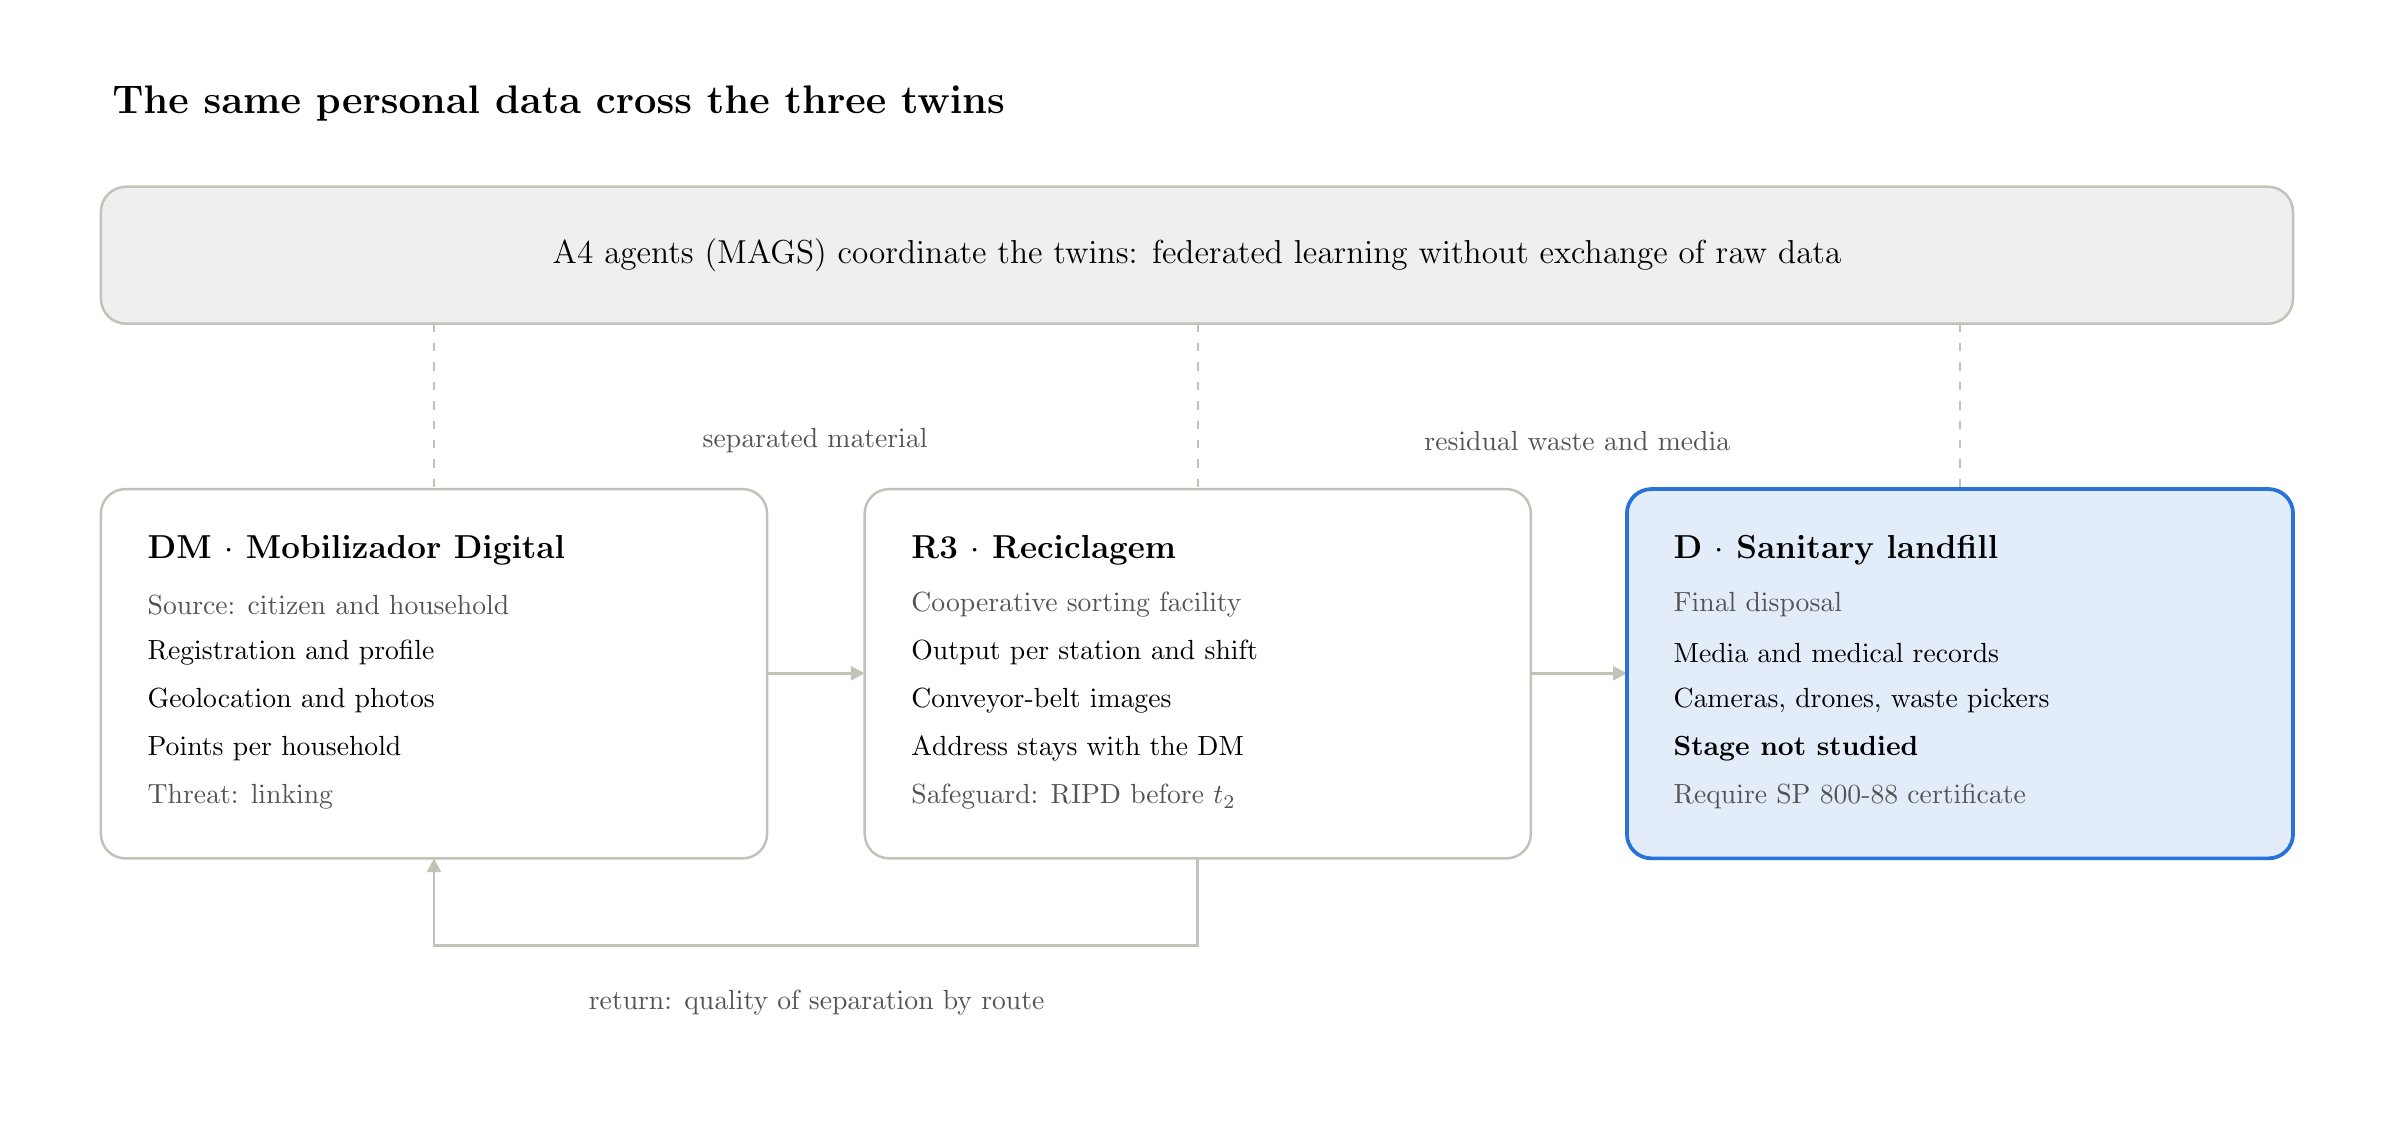
\begin{tikzpicture}[x=1cm,y=1cm]
  \path[use as bounding box] (0,0) rectangle (29.7,13.6);

  % Title and coordination of the three twins.
  \node[anchor=west,font=\bfseries\Large] at (0.95,12.64)
    {The same personal data cross the three twins};
  \draw[fill=cinzaBarra,draw=contorno,line width=0.9pt,rounded corners=0.32cm]
    (0.93,9.84) rectangle (28.77,11.58);
  \node[font=\large] at (14.85,10.71)
    {A4 agents (MAGS) coordinate the twins: federated learning without exchange of raw data};

  % Links from the coordination layer to each stage.
  \foreach \x in {5.16,14.86,24.54} {
    \draw[draw=contorno,line width=0.75pt,dash pattern=on 3pt off 4pt]
      (\x,9.84) -- (\x,7.74);
  }

  % Main flow and information return.
  \draw[draw=contorno,line width=1.1pt,-{Triangle[length=5pt,width=5pt]}]
    (9.39,5.40) -- (10.63,5.40);
  \draw[draw=contorno,line width=1.1pt,-{Triangle[length=5pt,width=5pt]}]
    (19.09,5.40) -- (20.31,5.40);
  \draw[draw=contorno,line width=1.0pt,-{Triangle[length=5pt,width=5pt]}]
    (14.86,3.05) -- (14.86,1.94) -- (5.16,1.94) -- (5.16,3.05);

  % Boxes of the three stages.
  \draw[draw=contorno,line width=0.9pt,rounded corners=0.31cm]
    (0.93,3.05) rectangle (9.39,7.74);
  \draw[draw=contorno,line width=0.9pt,rounded corners=0.31cm]
    (10.63,3.05) rectangle (19.09,7.74);
  \draw[fill=azulFundo,draw=azulContorno,line width=1.35pt,rounded corners=0.31cm]
    (20.31,3.05) rectangle (28.77,7.74);

  % Labels over the transitions.
  \node[font=\normalsize,text=cinzaTexto] at (10.00,8.35) {separated material};
  \node[font=\normalsize,text=cinzaTexto] at (19.68,8.35) {residual waste and media};

  % DM -- Digital Mobilizer.
  \node[anchor=west,font=\bfseries\large] at (1.40,6.96) {DM $\cdot$ Mobilizador Digital};
  \node[anchor=west,text=cinzaTexto] at (1.40,6.27) {Source: citizen and household};
  \node[anchor=west] at (1.40,5.66) {Registration and profile};
  \node[anchor=west] at (1.40,5.05) {Geolocation and photos};
  \node[anchor=west] at (1.40,4.44) {Points per household};
  \node[anchor=west,text=cinzaTexto] at (1.40,3.83) {Threat: linking};

  % R3 -- Recycling.
  \node[anchor=west,font=\bfseries\large] at (11.10,6.96) {R3 $\cdot$ Reciclagem};
  \node[anchor=west,text=cinzaTexto] at (11.10,6.27) {Cooperative sorting facility};
  \node[anchor=west] at (11.10,5.66) {Output per station and shift};
  \node[anchor=west] at (11.10,5.05) {Conveyor-belt images};
  \node[anchor=west] at (11.10,4.44) {Address stays with the DM};
  \node[anchor=west,text=cinzaTexto] at (11.10,3.83)
    {Safeguard: RIPD before $t_2$};

  % D -- Sanitary landfill.
  \node[anchor=west,font=\bfseries\large] at (20.78,6.96) {D $\cdot$ Sanitary landfill};
  \node[anchor=west,text=cinzaTexto] at (20.78,6.27) {Final disposal};
  \node[anchor=west] at (20.78,5.66) {Media and medical records};
  \node[anchor=west] at (20.78,5.05) {Cameras, drones, waste pickers};
  \node[anchor=west,font=\bfseries] at (20.78,4.44) {Stage not studied};
  \node[anchor=west,text=cinzaTexto] at (20.78,3.83)
    {Require SP 800-88 certificate};

  \node[font=\normalsize,text=cinzaTexto] at (10.02,1.22)
    {return: quality of separation by route};
\end{tikzpicture}
\end{document}
